\documentclass[xcolor=table, 11pt, aspectratio=169]{beamer}

%\usepackage{arev}
\usepackage{amsmath,amssymb,amscd}
\usepackage{dsfont}
\usepackage{mathrsfs}
\usepackage{yfonts}
\usepackage{bm}
\usepackage{graphicx}
\usepackage{tabularx}
\usepackage{animate}
%\usepackage{mathtools}
%\usepackage{ifthen}

%\usepackage{xeCJK}
%\usepackage{fontspec}
%\newfontfamily\cjkfont{PingFang SC}
%\setCJKmainfont{PingFang SC}
\newcolumntype{x}{>{\centering\arraybackslash}X}
\renewcommand{\arraystretch}{1.5}
\newcommand{\uone}{\mathrm U(1)}
\DeclareMathOperator{\img}{img}

\usepackage{tikz}
	\usetikzlibrary{calc}
	\usetikzlibrary{arrows,shapes, positioning, matrix}
	\usetikzlibrary{decorations.markings}
	\tikzset{>=stealth}
	\tikzstyle arrowstyle=[scale=1]
	\tikzstyle directed=[postaction={decorate,decoration={markings,
 	   mark=at position .15 with {\arrow[arrowstyle]{stealth}}}}]
\tikzstyle string=[thick,postaction={decorate,decoration={markings,
    mark=at position .55 with {\arrow[arrowstyle]{stealth}}}}]
\tikzstyle dual_string=[dashed,postaction={decorate,decoration={markings,
    mark=at position .55 with {\arrow[arrowstyle]{stealth}}}}]

\tikzstyle dw=[thick,postaction={decorate,decoration={markings,
    mark=at position 1 with {\arrow[arrowstyle]{stealth}}}}]
\tikzstyle group=[mbg]
\newcommand*{\halfway}{0.5*\pgfdecoratedpathlength+.5*8pt}\tikzstyle arrowstyle=[scale=1]
\newcommand*{\halfwayb}{0.5*\pgfdecoratedpathlength}
\tikzstyle arrowstyle=[scale=1]
\tikzstyle fermion=[thick,postaction={decorate},decoration={markings,
    mark=at position \halfway with {\arrow[arrowstyle]{latex}}}]
\tikzstyle fermion2=[thick,postaction={decorate},decoration={markings,
        mark=at position \halfwayb with {\arrow[arrowstyle]{latex}}}]

\usepackage{pgffor}
\newcommand{\mb}[1]{\mathbf{#1}}
\renewcommand{\cal}[1]{\mathcal{#1}}

\newcommand{\ag}[2]{#1_\mb{#2}}
\newcommand{\cohosub}[1]{\scalebox{0.72}{\textswab{#1}}}
\newcommand{\cohosubsub}[1]{\scalebox{0.6}{\textswab{#1}}}
\newcommand{\coho}[1]{\textswab{#1}}

\DeclareMathOperator{\tr}{Tr}
\DeclareMathOperator{\im}{Im}
\DeclareMathOperator{\re}{Re}

\mode<presentation>
{
  %\usetheme{Warsaw}
  % or ...
  %\useoutertheme{rectangle}
  \setbeamertemplate{frametitle}[default][center]
  \defbeamertemplate{itemize item}{flat}{\begin{pgfpicture}{-1ex}{0ex}{1ex}{2ex}
      \pgfpathcircle{\pgfpoint{0pt}{.6ex}}{0.6ex}
      \pgfusepath{fill}
    \end{pgfpicture}%
  }
  \defbeamertemplate{itemize subitem}{flat}{\footnotesize\raise0.5pt\hbox{\textbullet}}
  \defbeamertemplate{itemize subsubitem}{flat}{\footnotesize\raise0.5pt\hbox{\textbullet}}

  %\useinnertheme{circles}
  \setbeamertemplate{items}[flat]
  \setbeamertemplate{sections/subsections in toc}[circle]
  \setbeamertemplate{blocks}[rounded]
  \setbeamertemplate{title page}[default][colsep=-4bp,rounded=true]
  \setbeamertemplate{part page}[default][colsep=-4bp,rounded=true]
  \setbeamercovered{transparent}
  %\usecolortheme{spruce}
  %\definecolor{THU}{RGB}{116,61,130}
  \definecolor{mbg}{RGB}{0,0,160}
  \setbeamercolor*{palette primary}{fg=white,bg=mbg}
  \setbeamercolor*{titlelike}{parent=palette primary}
  \setbeamercolor*{structure}{fg=mbg}
  \setbeamercolor{frametitle}{fg=white,bg=mbg}
  % or whatever (possibly just delete it)
  \setbeamercolor{block title}{bg=mbg,fg=white}
  \setbeamercolor{block body}{bg=mbg!15}


  \addtobeamertemplate{navigation symbols}{}{ \hspace{1em}%
    \usebeamerfont{footline}%
    \insertframenumber / \inserttotalframenumber }
}


%\usepackage[english]{babel}
% or whatever

%\usepackage[latin1]{inputenc}
% or whatever

%\usepackage{times}
%\usepackage[T1]{fontenc}
% Or whatever. Note that the encoding and the font should match. If T1
% does not look nice, try deleting the line with the fontenc.

\title[Space-group SPTs] % (optional, use only with long paper titles)
{Classifying topological crystalline states in interacting fermionic systems: a roadmap}

\author[Y Qi] % (optional, use only with lots of authors)
{Yang~Qi}
% - Give the names in the same order as the appear in the paper.
% - Use the \inst{?} command only if the authors have different
%   affiliation.

\institute[Fudan] % (optional, but mostly needed)
{Department of Physics, Fudan University}
% - Use the \inst command only if there are several affiliations.
% - Keep it simple, no one is interested in your street address.

%\date{2016 Annual Meeting of Fudan CFTPP} % (optional, should be abbreviation of conference name)
%{Fudan University, Oct 13 2015}
%\date{Hong Kong Forum of Physics, HKU, Jan 7-9, 2019.}
%\date{QuIST V, Kunming, Aug. 2nd, 2019.}
%\date{Perimeter Institute, Sept. 3rd, 2019.}
%\date{Beihang University, Oct. 22nd, 2019.}
\date{QuIST VI, Chongqing, May 2021.}
% - Either use conference name or its abbreviation.
% - Not really informative to the audience, more for people (including
%   yourself) who are reading the slides online

\subject{Theoretical Physics}
% This is only inserted into the PDF information catalog. Can be left
% out.



% If you have a file called "university-logo-filename.xxx", where xxx
% is a graphic format that can be processed by latex or pdflatex,
% resp., then you can add a logo as follows:

\pgfdeclareimage[height=1cm]{university-logo}{../resources/fudan}
\logo{\pgfuseimage{university-logo}}

\AtBeginSection[]
{
\begin{frame}{Outline}
%	\begin{columns}
%		\begin{column}[t]{.45\textwidth}
%		\begin{center}
%			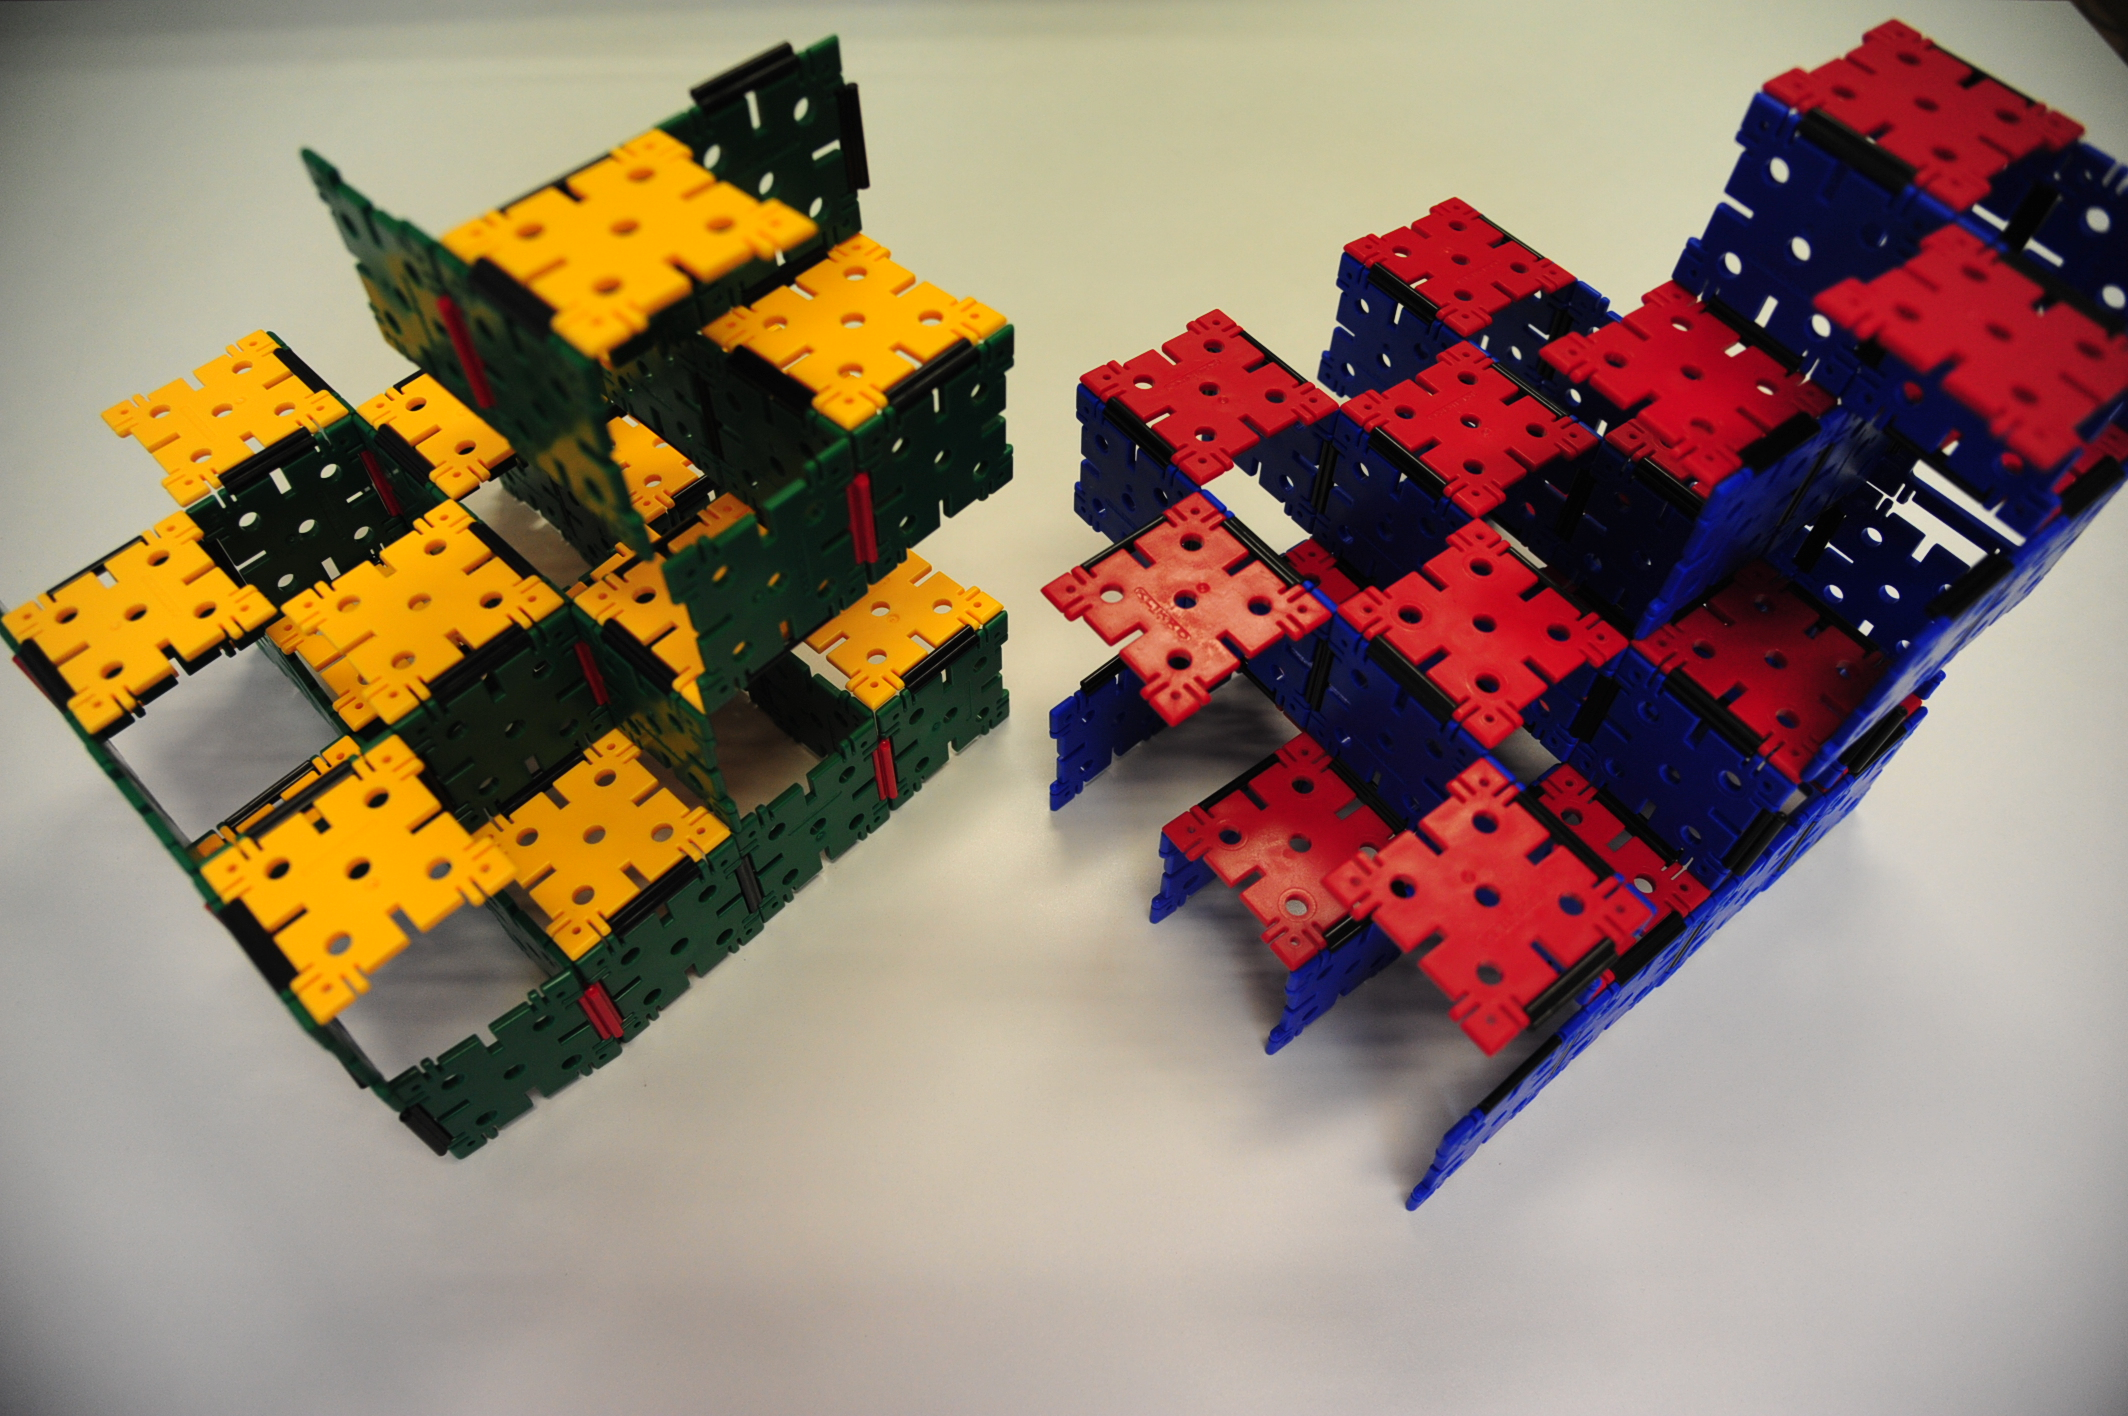
\includegraphics[height=4cm]{toys}
%		\end{center}
%	\end{column}
%	\begin{minipage}[t][0.5\textheight]{0.55\textwidth}
      \tableofcontents[currentsection]
%    \end{minipage}\hfill
%	\end{columns}
\end{frame}
}


% Delete this, if you do not want the table of contents to pop up at
% the beginning of each subsection:

\begin{document}

\begin{frame}
  \titlepage
\end{frame}

\begin{frame}{Collaborators}
  \begin{itemize}
  \item Yunqing Ouyang: Fudan University.
  \item Zhi-Da Song: Princeton University $\Rightarrow$ Beijing University.
  \item Chen Fang: Institute of Physics, Beijing.
  \item Zhengcheng Gu: Chinese University of Hong Kong.
    \begin{center}
      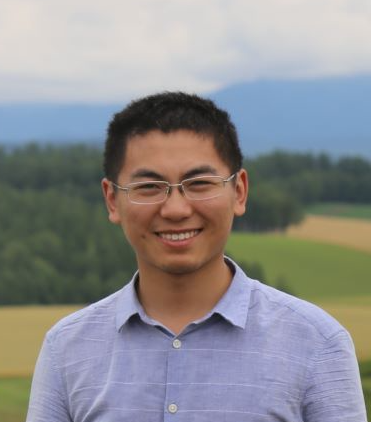
\includegraphics[height=3cm]{../people/zhidasong}
      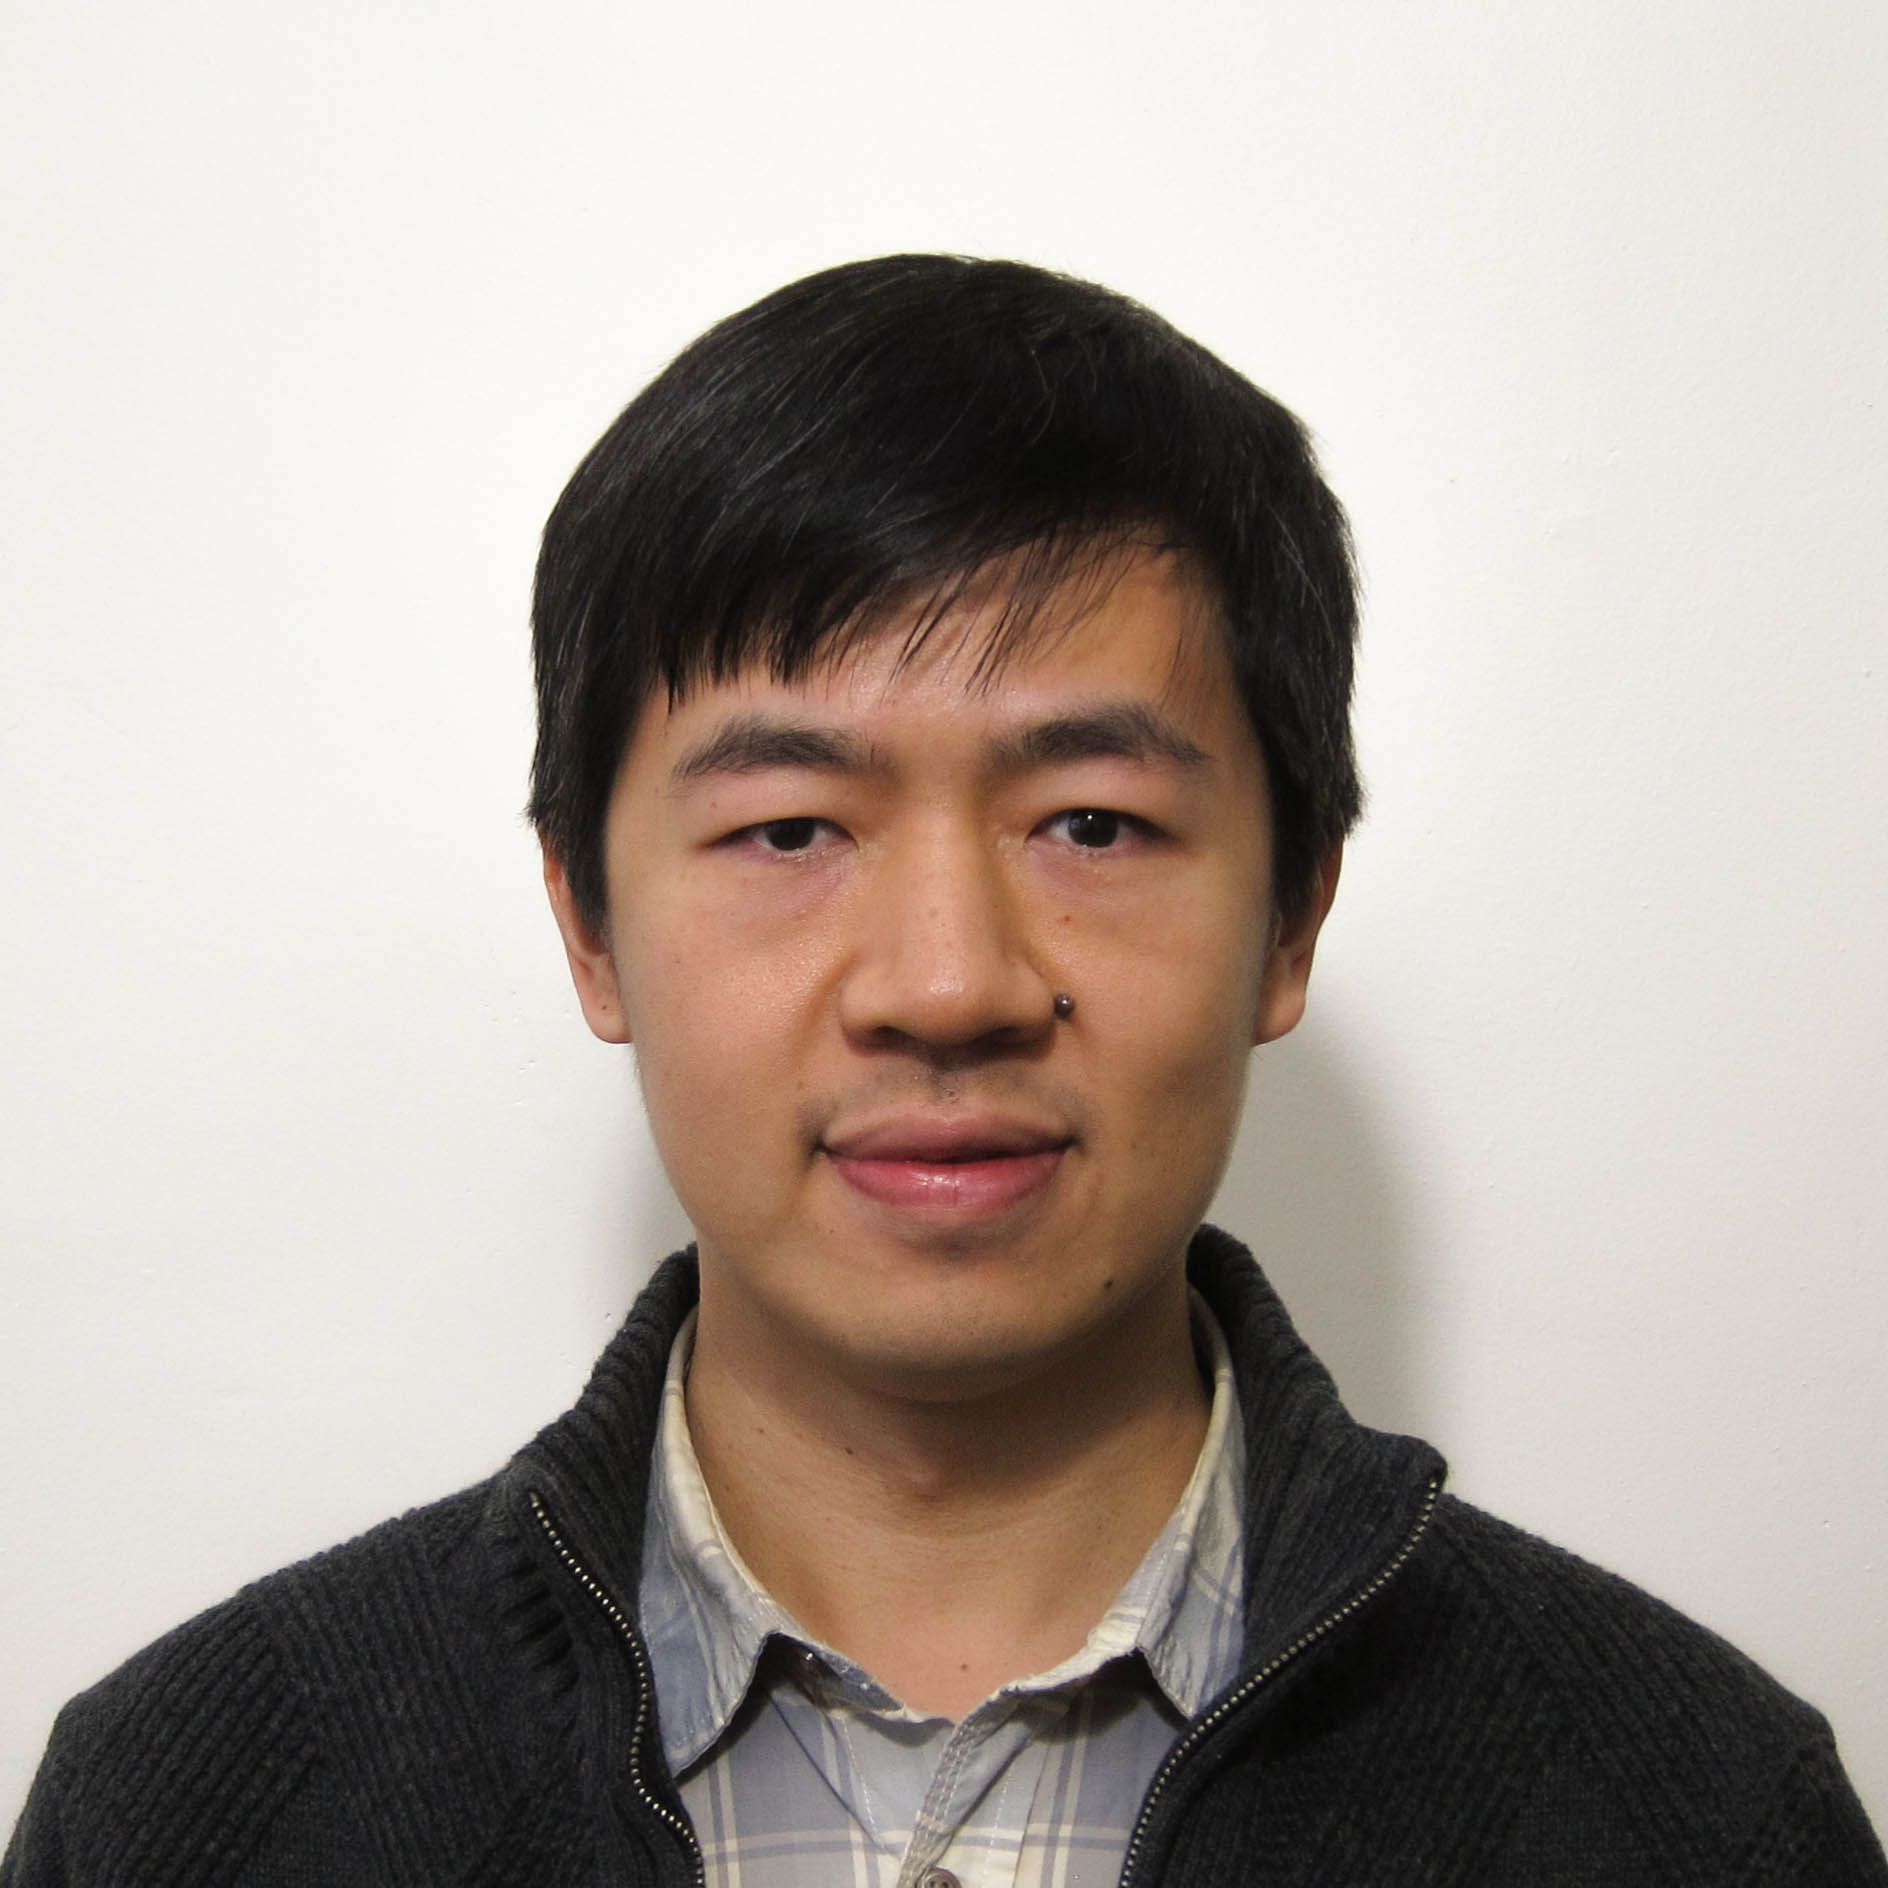
\includegraphics[height=3cm]{../people/chenfang}
    \end{center}
  \item Zhida Song, Chen Fang and Yang Qi, Nature Communications 11 4197 (2020).
  \item Yunqing Ouyang, Qing-Rui Wang, Zheng-Cheng Gu and Yang Qi, arXiv:2005.06572.
  \item Jian-Hao Zhang, Shuo Yang, Yang Qi and Zheng-Cheng Gu, 2012.15657.
\end{itemize}
\end{frame}

\begin{frame}{Outline}
%	\begin{columns}
%		\begin{column}[t]{.45\textwidth}
%		\begin{center}
%			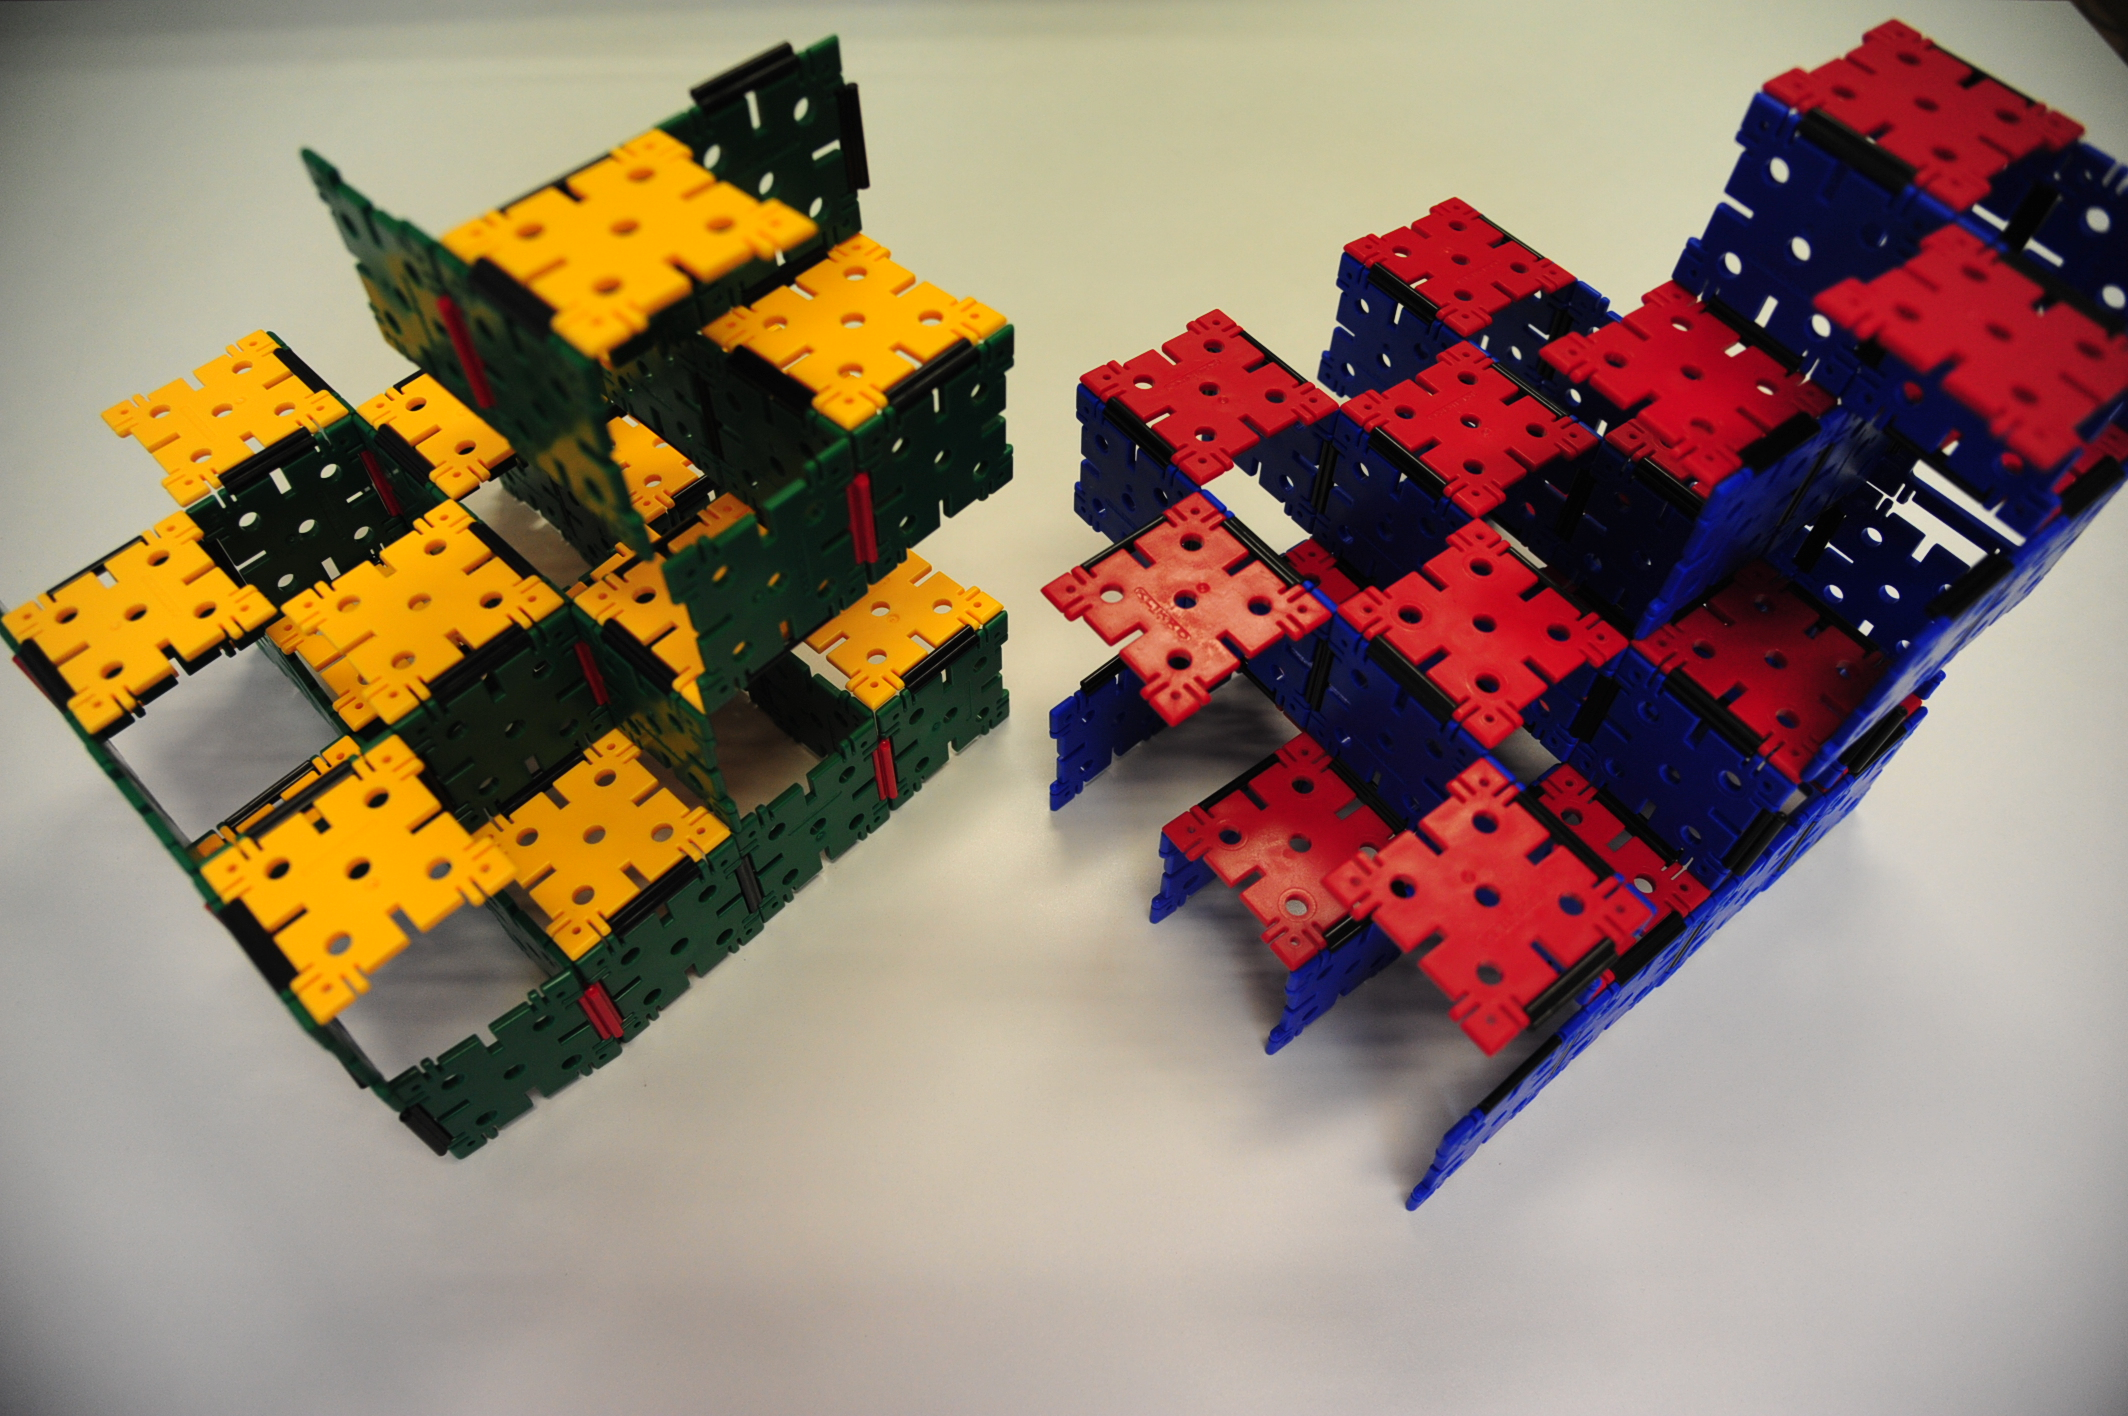
\includegraphics[height=4cm]{toys}
%		\end{center}
%	\end{column}
%	\begin{minipage}[t][0.5\textheight]{0.55\textwidth}
      \tableofcontents
%    \end{minipage}\hfill
%	\end{columns}
\end{frame}


\section{Introduction to SPT States}

\begin{frame}
  \frametitle{Symmetry-Protected Topological (SPT) states}
\begin{itemize}
\item SPT: gapped topological phases beyond Landau paradiam.
\item Gapped bulk : cannot be smoothly connected to a trivial state without closing gap or breaking symmetry.
\item Symmetry-protected gapless surface states.
\item Free-fermion states: topological insulators, topological superconductors: $K$-theory.
\item Bosonic SPTs: Haldane chain, CZX/Levin-Gu state, etc: Group Cohomology.
\item Interacting fermionic SPTs.
\end{itemize}
\end{frame}

\begin{frame}
  \frametitle{Abelian-group classification}
  \begin{itemize}
  \item SPT phases and boundary anomalies are classified by Abelian groups ($\mathbb Z$ or $\mathbb Z_n$).
    \begin{itemize}
    \item Addition: stacking of phases/gapless boundaries.
    \item 0: The trivial phase/gapped boundary.
    \end{itemize}
  \item 2D Chern-insulators (Integer Quantum Hall):
    \begin{center}
      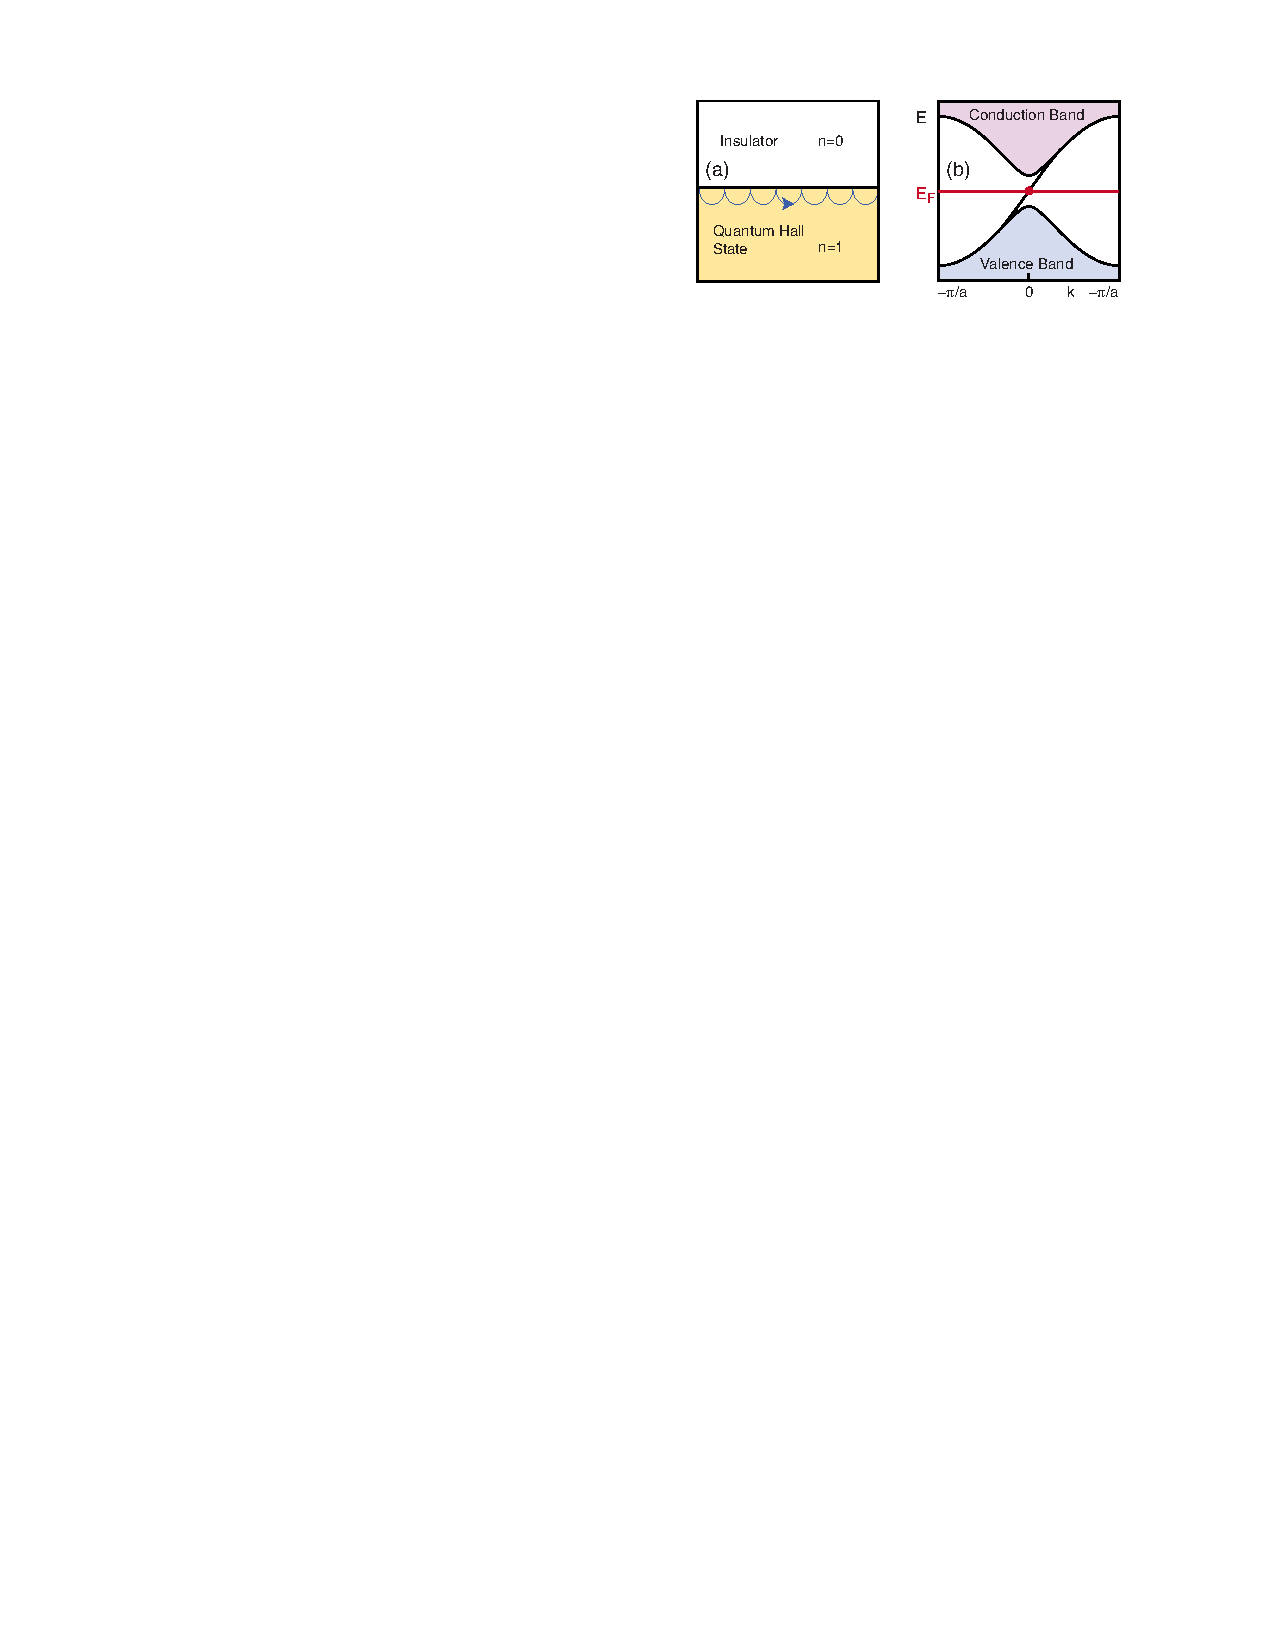
\includegraphics[width=8cm]{qhe_edge}
    \end{center}
    Classified by $\mathbb Z$: $[n]+[m]=[n+m]$; $[n]+[-n] = 0$.
  \end{itemize}
\end{frame}

\begin{frame}
	\frametitle{Abelian-group classification}
	\begin{itemize}
		\item 3D Topological Insulators:
		\begin{center}
			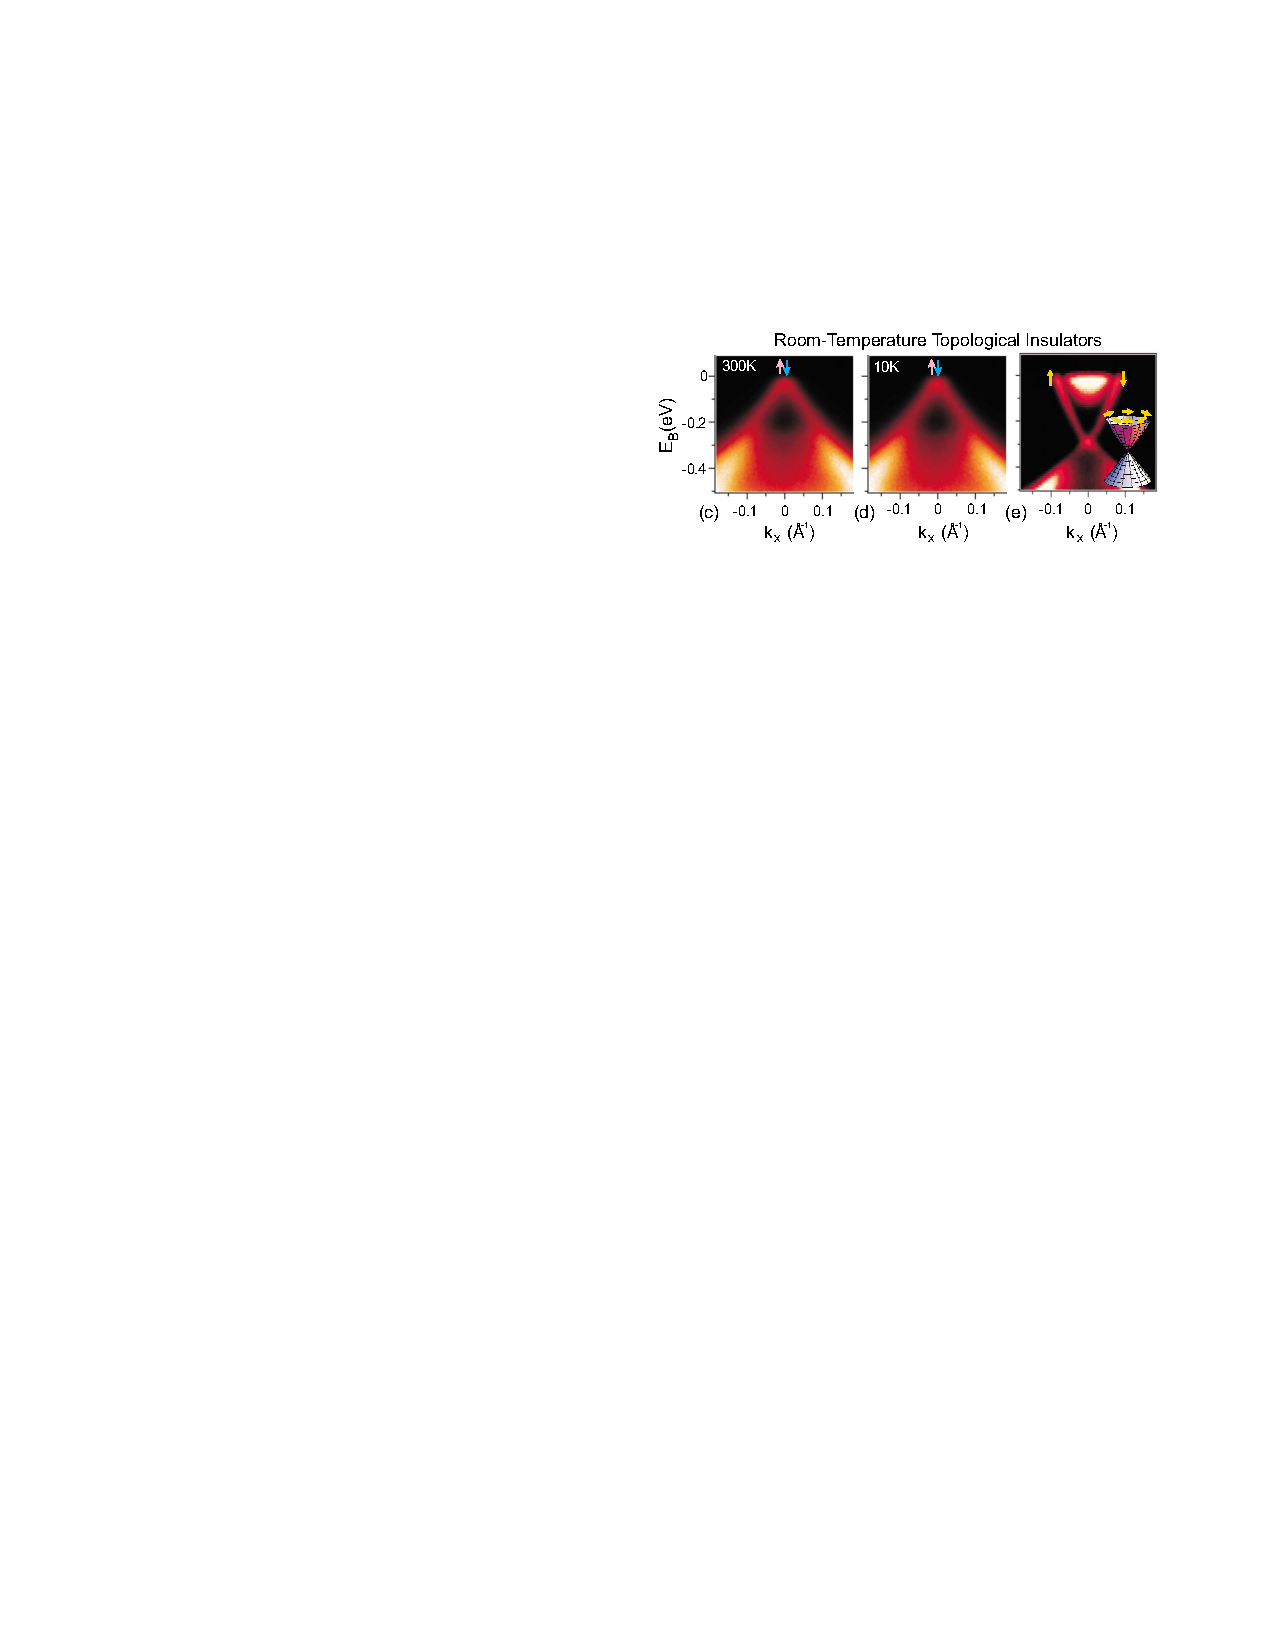
\includegraphics[width=8cm]{ti_surface}
		\end{center}
		Classified by $\mathbb Z_2$: $[1]+[1] = 0$.
		\item 1D Haldane chain:
		\begin{center}
			
\includegraphics[width=6cm]{../dimer/weak3d_aklt_blue}
		\end{center}
		Classified by $\mathbb Z_2$: $[1]+[1] = 0$.
	\end{itemize}
\end{frame}

\begin{frame}
\frametitle{Space-group SPT}
\begin{itemize}
\item We consider $G/G_0 = SG$.
\item Thorngren and Else (2018): the crystalline equivalence principle
\[H^{d+1}[G, \uone_{PT}].\]
\item Dimensional reduction: Liang Fu, Michael Hermele et al.\\
\emph{Examples: mirror SPT, weak SPT (translation symmetry).}
\item Patch construction: Zhida Song, Shengjie Huang, Yang Qi, Chen Fang and Michael Hermele, arXiv:1810.02330.
\item A more general construction for bosonic SPTs w/ all possible $G$.
\end{itemize}
\begin{center}
\begin{tikzpicture}[scale=.9]
\fill [blue!20] (0,0)--(1,1)--(1,3)--(0,2)--(0,0);
\draw (0,0)--(0,2)--(1,3);
\draw (-1.5,0)--(1.5,0)--(1.5,2)--(-1.5,2)--(-1.5,0);
\draw (1.5,0)--(2.5,1)--(2.5,3)--(1.5,2);
\draw (2.5,3)--(-.5,3)--(-1.5,2);
\end{tikzpicture}
\hspace{2em}
\begin{tikzpicture}[scale=.9]
\fill [blue!40,opacity=.5] (0,0)--(1,1)--(1,3)--(0,2)--(0,0);
\draw (0,0)--(0,2)--(1,3);
\fill [blue!40,opacity=.5] (.5,0)--(1.5,1)--(1.5,3)--(0.5,2)--(0.5,0);
\draw (.5,0)--(.5,2)--(1.5,3);
\fill [blue!40,opacity=.5] (1,0)--(2,1)--(2,3)--(1,2)--(1,0);
\draw (1,0)--(1,2)--(2,3);
\fill [blue!40,opacity=.5] (-.5,0)--(.5,1)--(.5,3)--(-0.5,2)--(-0.5,0);
\draw (-.5,0)--(-.5,2)--(.5,3);
\fill [blue!40,opacity=.5] (-1,0)--(0,1)--(0,3)--(-1,2)--(-1,0);
\draw (-1,0)--(-1,2)--(0,3);
\draw (-1.5,0)--(1.5,0)--(1.5,2)--(-1.5,2)--(-1.5,0);
\draw (1.5,0)--(2.5,1)--(2.5,3)--(1.5,2);
\draw (2.5,3)--(-.5,3)--(-1.5,2);
\end{tikzpicture}
\end{center}
\end{frame}

\section{Approach I: use crystalline equivalence principle}

\begin{frame}
  \frametitle{Crystalline equivalence principle}
  \begin{itemize}
  \item SPT classification remains the same if crystalline symmetry operations are replaced by onsite symmetry operations with the same group structure, provided:
    \begin{enumerate}
    \item Symmetries reversing space orientation $\Rightarrow$ antiunitary symmetries. (such as mirror reflection, glide plane, etc.)
    \item For fermions: spinless/spin-$\frac12$ $\Rightarrow$ spin-$\frac12$/spinless.
    \end{enumerate}
  \item We can compute crystalline-SPT as onsite-SPTs.
    \item Large symmetry groups (space groups are infinite): need an efficient algorithm.
  \end{itemize}
\end{frame}

\begin{frame}
	\frametitle{Fermionic SPT: a generalized cohomology theory}
	\begin{itemize}
        \item An Atiyah–Hirzebruch Spectral Sequence: an fSPT state is specified by several layers.
          \[E^{pq}_2=H^p[G_b, H^q(\text{pt}, ??)]]\Rightarrow H^{p+q}(BG_b, ??).\]
        \item Example: 2D fSPT,
          \begin{enumerate}
          \item $n_1\in H^1[G, \mathbb Z_2]$: Majorana-chain decoration.
          \item $n_2\in C^2[G, \mathbb Z_2]$: Complex-fermion decoration.
          \item $\nu_3\in C^3[G, \uone]$: Bosonic phase factor.
          \item A real-space construction: Q-R Wang and Z-C Gu, PRX 2020.
          \end{enumerate}
	\end{itemize}
\end{frame}

\begin{frame}
	\frametitle{Fermionic SPT: a generalized cohomology theory}
	\begin{itemize}
		\item Obstruction functions: higher-page derivatives of the spectral sequence.
		\item Example: checking if $n_1\in H^1[G, \mathbb Z_2]$ is obstructed?
		\begin{enumerate}
			\item Check $\mathcal O_3[n_1] = \omega_2\cup n_1 + s_1\cup n_1\cup n_1$ vanishes.
			\item Find $n_2$ such that $dn_2 = \mathcal O_3[n1]$.
			\item Check $\mathcal O_4[n_2]$ vanishes.
			\begin{align*}\mathcal O_4(01234) = \frac12\big[\omega_2\cup n_2 + n_2\cup n_2 + n_2 \cup_1 dn_2 + \omega_2(013)dn_2(1234)\\ + dn_2(0124)dn_2(0234)\big]
			-\frac14\big\{dn_2(0123)[1-dn_2(0124)]\text{ (mod 2)}\big\}.
		\end{align*}
		\end{enumerate}
		This defines a map between cohomology classes
		$n_1\mapsto \mathcal O_4$.
		\item In theory, this is the end of the story. But in practice...
	\end{itemize}
\end{frame}

\begin{frame}
	\frametitle{Computational cost}
	\begin{itemize}
		\item Key step: solving the cocycle/coboundary equation; finding $\ker d^n$ and $\img d^{n-1}$.
		\item ``Diagonalizing'' the coboundary matrix $d^n$: Smith Normal Form.
		\item $d^n$ acts on $\alpha(g_1,\ldots,g_n)$: $(|G|-1)^n$-dimension.
		\item Complexity = $O(N^3)$, $N = (|G|-1)^n$.
		\item Quite expensive for large $G$ ($|G| > 16$); infinite for $|G|=\infty$ (wallpaper and space groups).
	\end{itemize}
	\begin{block}{Can we do better?}
		\begin{itemize}
			\item For bSPTs: $H^n[G,\uone]$ can be computed using simpler $BG$.
			\item What about fSPTs and other cases w/ complicated maps b/w cohomology groups?
		\end{itemize}
	\end{block}
\end{frame}

\section{Approach II: real-space construction}
%\section{Mathematical details}
\section{Conclusion}

\begin{frame}
\frametitle{Mathematical Proof: Real-Space Construction is Complete}
\begin{itemize}
\item Equivariant group cohomology:
\[H^{d+1}[G, \uone_{PT}]]\simeq H^{d+1}_G[X, \uone_{PT}].\]
Here $X\sim\text{pt}$ is a (non-free) $G$-complex. See Thorngren and Else, PRX (2018).
\item There is a spectral sequence:
\[E_1^{pq}=\bigoplus_{\sigma\in X_p/G}H^q[G_\sigma,\uone_T]\Rightarrow
H^{p+q}_G[X,\uone_{PT}]\simeq H^{p+q}[G, \uone_{PT}]].\]
See Kenneth S. Brown's book, Chapter VII.
\item The topological space $Y$ we used is the Poincar\'e dual of $X$: $E^{pq}_r\simeq E^{q-1}_{d-p,r}$
\end{itemize}
\begin{center}
	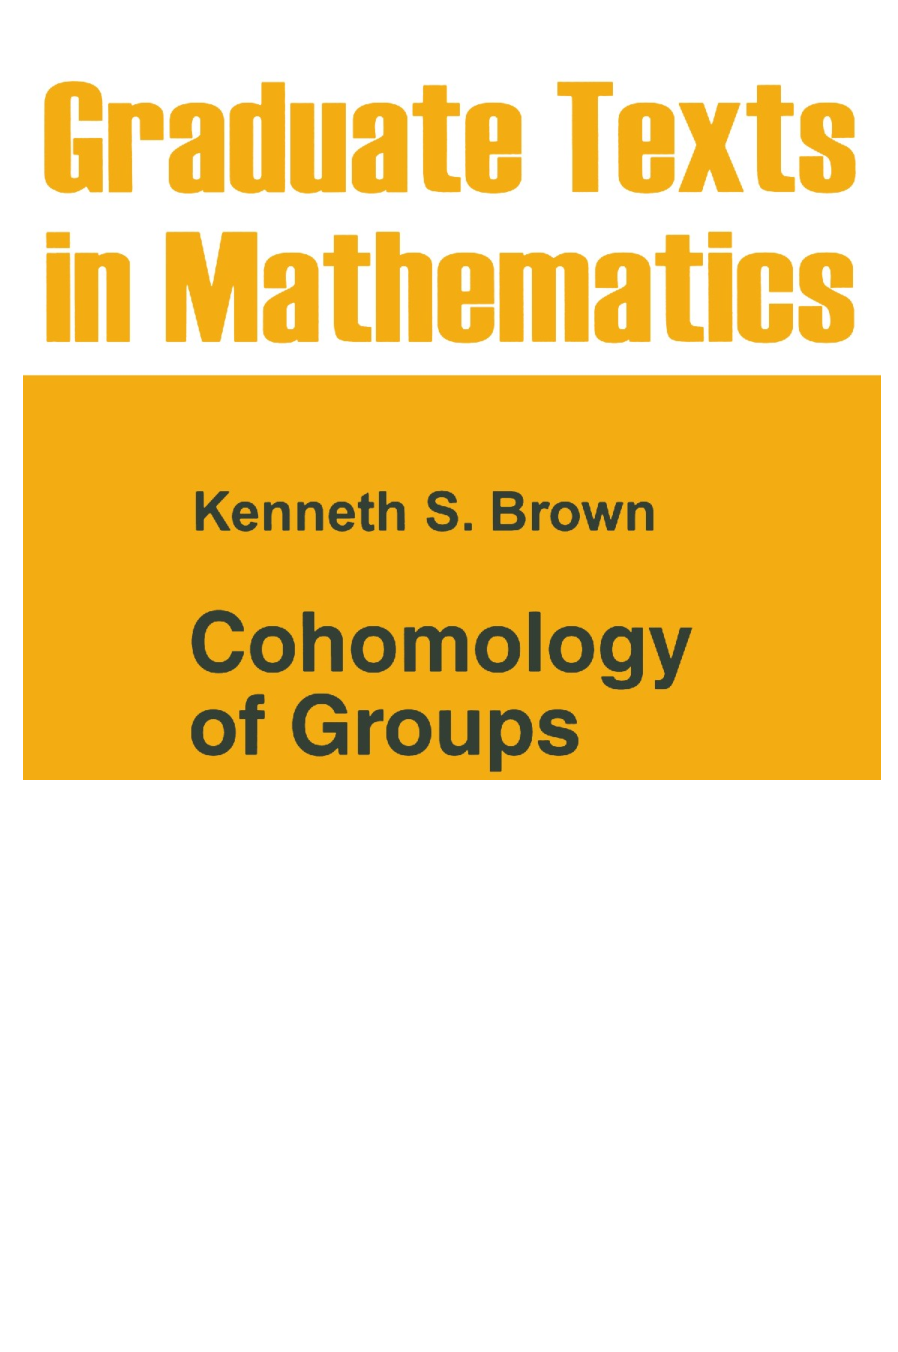
\includegraphics[height=2cm]{brown_book}
	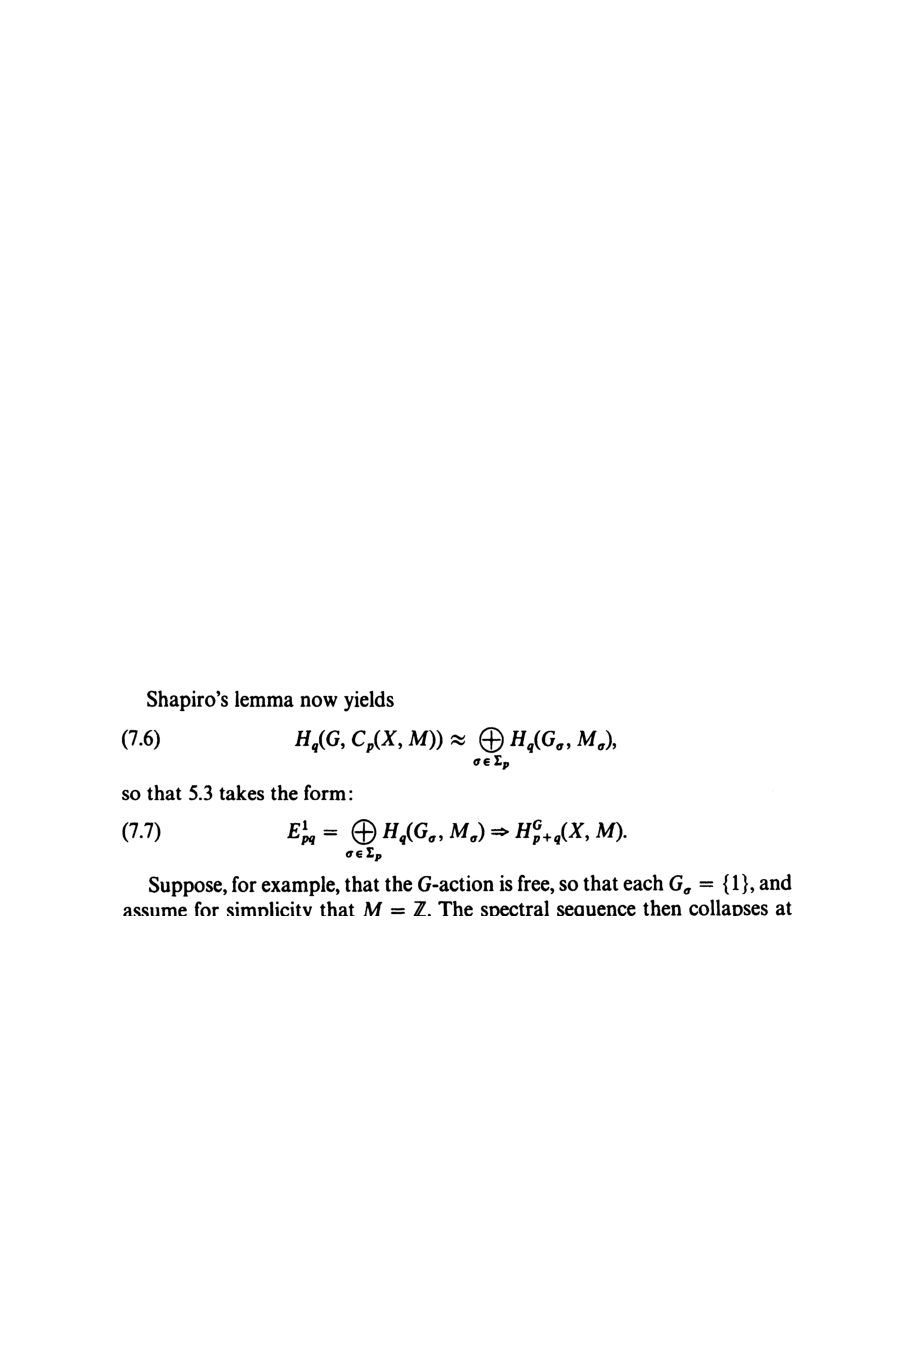
\includegraphics[height=2cm]{brown_ss}
\end{center}
\end{frame}

\begin{frame}
\frametitle{Summary}
\begin{itemize}
\item We develop a way to sysmetically construct space-group SPTs.
\item Check cocycle conditions and coboundary equivalences order-by-order.
\item For $G=SG\times G_0$, second page is enought.
\item Examples beyond simple layered construction.
\item Examples where second-page calculation is not enough.
\end{itemize}
\end{frame}

\begin{frame}
\frametitle{Outlooks}
\begin{itemize}
\item Outlook: cut-and-glue other things:
\begin{enumerate}
%\item Bosonic SPTs beyond group cohomology (E8 decorations).
\item Fermionic space-group SPTs.
\item 2D space-group SETs.
\end{enumerate}
\item A way to simplify computations for arbitrary symmetry groups.\\
See M Cheng and C Wang, arXiv:1810.12308.
\item Another work about spectral sequence: Ken Shiozaki, Masatoshi Sato and Kiyonori Gomi, arXiv:1802.06694 (momentum-space analysis).
\item An independent work: Else and Thorngren, arXiv:1810.10539.
\item Related work: K. Shiozaki, C. Zhaoxi Xiong, and K. Gomi,
arXiv:1810.00801.
\end{itemize}
\end{frame}

\end{document}
